\documentclass{llncs}
%
%
%espero que no se enfaden por incluir este paquete:
\usepackage{amsmath}
\usepackage{amssymb}
%\usepackage{amsthm}

\usepackage[dvips]{graphicx}
\usepackage{makeidx}  % allows for indexgeneration
\usepackage{color}
\usepackage[table]{xcolor}

\hyphenation{pro-per-ties}
\hyphenation{ge-ne-ral-ly}
\hyphenation{pre-fe-ren-ces}
\hyphenation{u-sing}
\hyphenation{pu-nish-ment}
\newcommand{\Pow}{\mathcal{P}}
\newcommand{\N}{\operatorname{N}}
\newcommand{\bool}{\operatorname*{\mathcal{B}}}
\newcommand{\Pos}{\operatorname{Pos}}
\newcommand{\Nec}{\operatorname{Nec}}
\newcommand{\Open}{\operatorname{Open}}
\newcommand{\Rp}{\operatorname{Rp}}
\newcommand{\Rn}{\operatorname{Rn}}
\newcommand{\FB}{\operatorname{FB}}
\newcommand{\UC}{\operatorname{UC}}
\newcommand{\T}{\mathcal{T}}
\newcommand{\Rel}{\mathcal{R}}
\newcommand{\C}{\mathcal{C}}
\newcommand{\Nat}{\mathbb{N}}
\newcommand{\Boolean}{\mathbb{B}}
\newcommand{\Q}{\mathbb{Q}}
\newcommand{\R}{\mathbb{R}}
\newcommand{\Z}{\mathbb{Z}}
\newcommand{\Head}{\mathcal{H}}
\newcommand{\Body}{\mathcal{B}}
\newcommand{\Dom}{\mathcal{D}}
\newcommand{\INS}{\mbox{\textbf{insert}}}
\newcommand{\DEL}{\mbox{\textbf{delete}}}
\newcommand{\MOD}{\mbox{\textbf{modify}}}
\newcommand{\REV}{\mbox{\textbf{revise}}}
\newcommand{\Overlap}{\mbox{\textbf{Overlap}}}
\newcommand{\A}{\mathcal{A}}
\newcommand{\I}{\mathcal{I}}
\renewcommand{\Join}{\bowtie}
%\theoremstyle{definition}
%\newtheorem{definition}{Definition}
\begin{document}

\mainmatter              % start of the contributions
%
\title{Data Manipulation Language for fuzzy temporal databases.}
%
%\titlerunning{A Fuzzy Valid-Time Model}  % abbreviated title (for running head)
%                                     also used for the TOC unless
%                                     \toctitle is used
%
\author{Jos\'e Enrique Pons \and Olga Pons Capote}
%Jeffrey Dean \and David Grove \and Craig Chambers \and Kim~B.~Bruce \and
%Elsa Bertino}
%
\authorrunning{Jos\'e Enrique Pons et al.} % abbreviated author list (for running head)
%
%%%% list of authors for the TOC (use if author list has to be modified)
%\tocauthor{Ivar Ekeland, Roger Temam, Jeffrey Dean, David Grove,
%Craig Chambers, Kim B. Bruce, and Elisa Bertino}
%
\institute{
Department of Computer Science and Artificial Intelligence \\
Universidad de Granada \\
Escuela T\'ecnica Superior de Ingenier\'ia Inform\'atica \\
C/Periodista Daniel Saucedo Aranda s/n \\
E-18071 (Granada-Spain)\\
\email{jpons,opc@decsai.ugr.es}\\ 
%WWW home page:
%\texttt{http://users/\homedir iekeland/web/welcome.html}
%\and
%Universit\'{e} de Paris-Sud,
%Laboratoire d'Analyse Num\'{e}rique, B\^{a}timent 425,\\
%F-91405 Orsay Cedex, France
}

\maketitle              % typeset the title of the contribution

\begin{abstract}

\end{abstract}


\section{\label{sec:preliminaries}Preliminares}

% \begin{definition}
%  \label{def:temporal-schema}
% A crisp temporal schema is given by the following:
% 
% \begin{equation}
% \label{eq:temporal-relation}
% R = \left(A_1, \ldots, A_n, T_s, T_e \right) 
% \end{equation}
% Where $A_1, \ldots, A_n$ are the attributes of the relation $R$ and $T = \left \lbrace T_s, T_e\right \rbrace$ is the staring and ending points of the valid-time interval.
% We define $r$ as an instance of the relation $R$.
% \end{definition}


\begin{definition}
\label{def:valid-time-relation}
\emph{Valid-time relation.}
Consider the following definitions and notations:

\begin{itemize}
 \item A set of non-temporal attributes.
	\begin{equation}
	\label{eq:attribute-set}
	A = \left \lbrace A_1, A_2, \ldots, A_n \right \rbrace
	\end{equation}
      The domain for each attribute $A_1, \ldots, A_n$ is $D_1, \ldots, D_n$ respectively. 
\item The original primary key $A_K$ is a subset of the attributes in $A$.
      \begin{equation}
       \label{eq:primary-key-a}
      A_K \subseteq A
      \end{equation}
\item Two attributes, $S$  and $E$ for the starting and ending points respectively. $I$ defines the valid time interval for the data. 
\begin{equation}
 \label{eq:attribute-time-interval}
I = \left \lbrace S, E \right \rbrace
\end{equation}

$\T$ is the time domain.

\item Then $R$, the schema for the valid-time relation is:
\begin{equation}
 \label{eq:valid-time-relation}
R = A \cup  I
\end{equation}
\item The primary key for the valid-time relation $R$ is:
\begin{equation}
 \label{eq:valid-time-temporal-pk}
PK = A_K \cup I
\end{equation}


\item We will note by $r$ any valid instance of $R$. 
      \begin{equation}
       \label{eq:valid-time-instance}
      r \subseteq D_1\ x\ \ldots\ x\ D_n x\ T x\ T
      \end{equation}


     % \end{itemize}
\item $V(t)$ is the set of all the versions for a given tuple $t$. Formally,

\begin{equation}
 \label{eq:all-the-versions}
V(t) =\left \lbrace t_i \in r, t_i\left[A_K\right] = t\left[A_K\right] \right \rbrace
\end{equation}
Obviously, $t$ itself is included in the set.
% If a tuple $t$ contains more than one version, the result of $Vt$ is a set. We will use the index $k$ to address the elements of the set. E.g. $Vt = \left \lbrace t_1, t_2, \ldots, t_n \right \rbrace$. Then $t_k , k \in \left \lbrace 1, \ldots, n \right \rbrace$ is an element of $Vt$.
\end{itemize}
\end{definition}
We will illustrate the definitions with an example.

\begin{example}
Consider the set of attributes $A = \left \lbrace A_1, A_2, A_3 \right \rbrace$. The primary key for these attributes is given by $A_K = \left \lbrace A_1, A_2 \right \rbrace$. Let $I = \left \lbrace S, E \right \rbrace$ be the set of temporal attributes that define the validity period of the data. $R$ is the valid-time relation and $r$ is an instance of the relation. The instance $r$ is given by the following elements. $r = \left \lbrace \left(a_{11}, a_{12}, a_{13}, s_1 ,e_1 \right) \right.$,  $\left(a_{21}, a_{22}, a_{23}, s_2, e_2 \right)$ , $\left. \left(a_{11}, a_{12}, a_{31}, s_3, e_3 \right) \right \rbrace$. The instance $r$ is illustrated in Table \ref{tbl:sample-definitions}. 
Consider the tuple $t_1 = \left(a_{11}, a_{12}, a_{13}, s_1 ,e_1 \right)$. Then,
\begin{align}
 \nonumber
 t_1\left[S \right]&=s_1\\
 \nonumber
t_1[E]&=e_1\\
 \nonumber
t_1[S,E]&= \left(s_1, e_1\right)\\
 \nonumber
t_1\left[A_K\right] &= \left(a_{11}, a_{12} \right) \\
 \nonumber
t_1\left[PK\right] &=\left(a_{11}, a_{12}, s_1, e_1\right)\\
 \nonumber
V(t_1) &= \left \lbrace t_1, t_3 \right \rbrace
\end{align}

\begin{table}
\centering
\label{tbl:sample-definitions}
\caption{Sample database containing the instance $r$ of the valid-time relation $R$.}
\begin{tabular}{c c c c c c}\\
\hline
& \textbf{A$_1$}  & \textbf{A$_2$}  & $A_3$ & $S$ & $E$ \\
\hline
$t_1$&$a_{11}$ & $a_{12}$ & $a_{13}$ & $s_1$ & $e_1$ \\
$t_2$ & $a_{21}$ & $a_{22}$ & $a_{23}$ &  $s_2$ & $e_2$ \\
$t_3$ & $a_{11}$ & $a_{12}$ & $a_{31}$ & $s_3$ & $e_3$\\
\hline\\
\end{tabular}
\end{table}


\end{example}

% \begin{definition}
%  \label{def:fuzzy-temporal-schema}
% A fuzzy temporal schema is given by the following:
% 
% % \begin{equation}
% %  \label{eq:fuzzy-temporal-relation}
% % R = \left(A_1, \ldots, A_n, T_s, T_e \right) 
% % \end{equation}
% % Where 
%  \end{definition}



\begin{definition}
\label{def:generalized-fuzzy-temporal-domain}
\emph{Generalized fuzzy temporal domain.}
Consider $\T$ to be the temporal domain, and let $\tilde \Pow\left( \T\right)$ be the set of all \emph{normalized} possibility distributions defined on $\T$.
The Generalized Fuzzy Temporal Domain, $\T_G$ is
\begin{equation}
\T_G \subseteq \left \lbrace \tilde \Pow\left( \T\right) \cup \text{NULL} \right \rbrace
\end{equation}
\end{definition}

Note that $\T_G \subseteq D_G$. The datatypes for this domain have been studied previously in section \ref{sec:time-rep} and are shown in tables \ref{tbl:time-point-types} and \ref{tbl:time-interval-types}.

A generalized fuzzy relation is defined in \cite{Medina1994}. Here, we will extend the definition to a generalized fuzzy temporal relation.

\begin{definition}
\emph{Generalized fuzzy temporal relation.}
\label{def:fuzzy-temporal-relation}
Consider the elements in definition \ref{def:valid-time-relation}. Some of them will be extended for the fuzzy case.

\begin{itemize}
%  \item A set of non-temporal fuzzy  or crisp attributes.
% 	\begin{equation}
% 	\label{eq:fuzzy-attribute-set}
% 	A = \left \lbrace A_1, A_2, \ldots, A_n \right \rbrace
% 	\end{equation}
%       The domain for each attribute $A_1, \ldots, A_n$ is $D_1, \ldots, D_n$ respectively. 
% \item The primary key $A_K$ is a subset of $A$.
%       \begin{equation}
%        \label{eq:fuzzy-primary-key-a}
%       A_K \subset A
%       \end{equation}
% A formal definition of primary key for fuzzy relational databases will be given later in Definition \ref{def:generalized-primary-key}.
% \item A set of two attributes; $S$  and $E$ the attributes for the starting and ending ill-known points respectively. $I$ is a possibilistic validity period \emph{PVP} as explained in Section \ref{subsec:ill-known-interval}.
% \begin{equation}
%  \label{eq:fuzzy-attribute-time-interval}
% I = \left \lbrace S, E \right \rbrace
% \end{equation}
\item An attribute called version identifier, $V_{ID}$, will be added to the schema. This attribute is a counter for each different version of the entities. 
% \begin{equation}
%  \label{eq:fuzzy-version-identifier}
% V_{ID} \subset \N
% \end{equation}



\item Then $R_{FTG}$, the schema for the fuzzy valid-time relation is:
\begin{equation}
 \label{eq:fuzzy-valid-time-relation}
R_{FTG} = A \cup V_{ID} \cup  I
\end{equation}
\item The primary key for the fuzzy valid-time relation $R_{FTG}$ is:
\begin{equation}
 \label{eq:fuzzy-valid-time-temporal-pk}
K_{GT} = A_K \cup V_{ID}
\end{equation}
A formal definition of the primary key for fuzzy valid-time relations will be given later in Definition \ref{def:generalized-fuzzy-temporal-key}.


\item We will note by $r$ any valid instance of $R_{FTG}$. 
      \begin{equation}
       \label{eq:fuzzy-valid-time-instance}
      r \subseteq D_1\ x\ \ldots\ x\ D_n x\ \mathbb{N}  x\  \T_G\  x\ \T_G 
      \end{equation}

% \item Let $t$ be a tuple in the instance $r$; $t \in r$:
%       \begin{itemize}
%       \item We will note the values for the starting and the ending  points,$s$ and $e$  respectively. The value for the time interval is given by $i$.
%       \begin{align}
%        \label{eq:fuzzy-starting-point}
%       s = t\left[S \right]\\
%       e = t\left[E \right]\\
%       i = \left(s, e\right)
%       \end{align}
% 
% 
%       \item Let $A_k \subset A$ be the set of the non-temporal attributes that are part of the primary key (equation \eqref{eq:fuzzy-primary-key-a}). Then, $a_k$ denotes the values for the non-temporal attributes of the primary key.
% 	    \begin{equation}
% 	     \label{eq:fuzzy-pk-attribute} 
% 	      a_k = t\left[A_K \right]
% 	    \end{equation}
% 
    \item Let $K_{GT}$ be the primary key for the valid-time relation as given in equation \eqref{eq:fuzzy-valid-time-temporal-pk}. Then, $k$ denotes the values for the attributes in the primary key.
	  \begin{equation}
	   \label{eq:fuzzy-value-pk}
	  k = t\left[K_{GT} \right]
	  \end{equation}
% 
% 
%       \end{itemize}
% \item $Vt$ is the set with all the versions for a given tuple $t$.
% 
% \begin{equation}
%  \label{eq:fuzzy-all-the-versions}
% Vt = r\left(t\left[A_K\right] \right)
% \end{equation}
% If a tuple $t$ contains more than one version, the result of $Vt$ is a set. We will use the index $k$ to address the elements of the set. E.g. $Vt = \left \lbrace t_1, t_2, \ldots, t_n \right \rbrace$. Then $t_k , k \in \left \lbrace 1, \ldots, n \right \rbrace$ is an element of $Vt$.
\end{itemize}
%\end{definition}

Table \ref{tbl:fuzzy-sample-definitions} contains an example instance.


\begin{table}
\caption{\label{tbl:fuzzy-sample-definitions}Sample database containing the instance $r$ of the fuzzy valid-time relation $R_{FTG}$.}
\centering
%\centerline{\small DATA TYPES}
\begin{tabular}{c c c c c c c}\\
\hline
& \textbf{A$_1$}  & \textbf{A$_2$}  & $A_3$ & $V_{ID}$ & $S$ & $E$ \\
\hline
$t_1$&$a_{11}$ & $a_{12}$ & $a_{13}$ & $001$ & $s_1$ & $e_1$ \\
$t_2$ & $a_{21}$ & $a_{22}$ & $a_{23}$& $001$ &  $s_2$ & $e_2$ \\
$t_3$ & $a_{11}$ & $a_{12}$ & $a_{31}$& $002$ & $s_3$ & $e_3$\\
\hline\\
\end{tabular}
\end{table}



% 
% 
% Consider $\A$ to be the set of all the entities, and let $A=\left(A_1, \ldots, A_n \right), A \in \A$ be the set of (fuzzy) attributes that define an entity. Let $\I_{PVP}$ be the set of all the ill-known time intervals and let $I = \left(X, Y \right)$ be a PVP, $I \in \I_{PVP}$.  The pair $\left(A, I\right)$ expresses that the data regarding the entity A are valid during the ill-known time interval I. Let $R_{FTG} \subseteq \A \  x\  \I_{PVP}$ be a valid-time relation. Then, the following equation indicates that the pair $\left(A, I\right)$ is in the relation R:
% 
% \begin{equation}
% \label{eq:fuzzy-rel-def}
% \left( R_{FTG}, \left(A , I\right) \right)
% \end{equation}
% 
 A generalized fuzzy temporal relation $R_{FTG}$ can be noted also by:
\label{def:generalized-fuzzy-temporal-relation}
\begin{equation}
\label{eq:generalized-fuzzy-temporal-relation}
R_{FTG} = \left(\Head, \Body \right)
\end{equation}
Where $\Head$ is the Head of the relation and consists on a fixed set of triplets attribute- domain - compatibility with an optional the valid-time attribute:

\begin{align}
\label{eq:head-valid-time}
\Head = \big \lbrace \left(A_{G1}:D_{G1}\left[,C_{A_{G1}} \right] \right),\\
\nonumber
 \ldots,\\
 \nonumber
  \left(A_{Gn}:D_{Gn}\left[,C_{A_{Gn}} \right] \right),\\
  \nonumber
  \Big[  \left( \text{PVP}, D_{\text{PVP}}\left[,C_{A_{\text{PVP}}} \right] \right) \Big] \big \rbrace
\end{align}
Note that $D_{Gj}$ ($j = 1, \ldots, n$) is the domain for the attribute $A_{Gj}$. $C_{A_{Gj}}$ is the compatibility attribute in the unit interval $\left[0, 1 \right]$.

$\Body$ is the body of the relation and it consists on a set of tuples. Each tuple is a set of triplets attribute- value- degree with an optional valid-time attribute:

\begin{align}
\label{eq:body-valid-time}
\Body = \big \lbrace \ldots \{ \left(A_{G1}:\tilde{d}_{i1}\left[,c_{i1} \right] \right),\\
\nonumber
 \ldots,\\
 \nonumber
  \left(A_{Gn}:\tilde{d}_{in}\left[,c_{in} \right] \right),\\
  \nonumber
   \Big[  \left( \text{PVP}, \tilde{d}_{\text{PVP}} \left[,C_{A_{\text{PVP}}} \right] \right)  \Big] \} \ldots \big \rbrace
\end{align}

\end{definition}







\section{\label{sec:selection}Selection}
The selection operator $\sigma$ obtain a subset of tuples that fulfill a set of constraints from a given relation $R$. The set of constraints is usually a boolean combination of atomic constraints. The selection operator is noted as follows:
\begin{equation}
 \label{eq:selection}
\sigma_{P} \left( R \right)
\end{equation}

Where $R$ is the relation, and $P$ is the selection formula. The selection formula is a set of two elements:
% \begin{itemize}
% \item relation.attribute boolean relation relation.attribute
% \item relation.temporal-attribute allen-relation relation.temporal-attribute 
% \end{itemize}
\begin{equation}
 \label{eq:selection_formula}
P = \left \lbrace Q, Q^{t}\right \rbrace
\end{equation}

Where $q$ is a boolean combination of (possibly) fuzzy (and bipolar) non-temporal constraints and $q^{t}$ is also a boolean combination of fuzzy temporal constraints.

\begin{equation}
 \label{eq:non-temporal-constraints}
Q = \left \lbrace q^{\left \lbrace \mbox{pos,neg} \right \rbrace}_{\mbox{attribute}_1}  \theta \mbox{ val }, \ldots, q^{\left \lbrace \mbox{pos,neg} \right \rbrace}_{\mbox{attribute}_n}  \theta \mbox{ val } \right \rbrace
\end{equation}
Where $\theta$ is an artihmetic operator; one of $\left \lbrace =, \neq, <, \leq, >, \geq \right \rbrace$ and val is a value in the domain of the attribute. 

Then, consider a boolean function $\bool:\Boolean^{n}  \rightarrow \Boolean$. The evaluation function for the constraints in $Q$  is given by:

\begin{equation}
 \label{eq:evaluation-function}
\lambda : Q \rightarrow \Boolean : \lambda (Q) \rightarrow \bool \left(q^{\left \lbrace \mbox{pos,neg} \right \rbrace}_{\mbox{attribute}_1}  \theta \mbox{ val }, \ldots, q^{\left \lbrace \mbox{pos,neg} \right \rbrace}_{\mbox{attribute}_n}  \theta \mbox{ val } \right)
\end{equation}

Now, the uncertainty about the evaluation of $Q$ and a boolean function $\bool:\Boolean^{n}  \rightarrow \Boolean$ is given by:

\begin{equation}
 \label{eq:evaluation-lambda-function}
\pi_{\lambda \left(Q \right)} = \tilde{\bool} \left(\pi_{q^{\left \lbrace \mbox{pos,neg} \right \rbrace}_{\mbox{attribute}_1}  \theta \mbox{ val }}, \ldots, \pi_{q^{\left \lbrace \mbox{pos,neg} \right \rbrace}_{\mbox{attribute}_n}  \theta \mbox{ val }} \right)
\end{equation}


The temporal constraints, $Q^t$ are provided in a similar way. The main difference is that, instead of comparations like $\left \lbrace =, \neq, <, \leq, >, \geq \right \rbrace$, we use the allen's relations. Hence, the representation of the temporal constraints is expressed as follows:

\begin{equation}
\label{eq:temporal-constratins}
Q^{t} = \left \lbrace q_{\mbox{attribute}_1}  ar \mbox{ val }, \ldots, q_{\mbox{attribute}_n}  ar \mbox{ val } \right \rbrace
\end{equation}
Here, $ar$ is one of the thirdteen Allen's relations (equal, before, overlaps, starts, finishes, meets, during) and their respective reverses.


Now the combination of temporal and non-temporal results should be explicited here.
\begin{example}
Consider an employee's database. The data are stored in two tables; Table \ref{table:employees} (relation $R$) contains temporal data about the employees and Table \ref{table:address} (relation $S$) contains temporal  data about the addresses for each emploree. Consider now that the user wants to obtain all the employees who are a profesor and that worked during the time interval $\left[7, 10 \right]$.
%\vspace{-10pt} \ref{table:employees} \ref{table:address}

\begin{table}
\centering
\caption{Employee's database. Relation $R$.}

\begin{tabular}{c c c c c c }
\hline
ID & Job & Works for & Start & Finish \\ \hline
1 & Prof. & 4 & 5 & 10 \\
2 & Tech. & 4 & 3 & 7 \\
3 & Account. & 4  & 4 & 10 \\
4 & Adm. & - & 1 & UC \\
1 & Prof. & 4 & 11 & UC \\
\hline 
\end{tabular}
\label{table:employees}

%\vspace{10pt}


\end{table}

%\vspace{-25pt}

%\vspace{-10pt}

\begin{table}
\centering
\caption{Address database. Relation $S$.}

\begin{tabular}{c c c c }
\hline
ID & Adr. & Start & Finish \\ \hline
1 & C/ Camino de ronda & FB & 12 \\
2 & C/ Recogidas & FB & UC \\ 
3 & C/ Pintor Maldonado & FB & UC \\
4 & C/ Mesones & FB & UC \\
1 & C/ Manuel de Falla & 12 & UC \\
\hline 
\end{tabular}
\label{table:address}

%\vspace{10pt}


\end{table}

%\vspace{-25pt}

The selection formula is the following:

\begin{equation}
 \label{eq:selection-example}
\sigma_{r.Job = 'Profesor', r.T \mbox{ During } \left[7, 10\right]} \left(R \right)
\end{equation}
The resultset for the selection is shown in Table \ref{table:example-selection}.
\end{example}

%\vspace{-10pt}

\begin{table}
\centering
\caption{Resultset table for the selection in equation \eqref{eq:selection-example}}

\begin{tabular}{c c c c c c }
\hline
ID & Job & Works for & Start & Finish \\ \hline
1 & Prof. & 4 & 5 & 10 \\
\hline 
\end{tabular}
\label{table:example-selection}

%\vspace{10pt}


\end{table}

%\vspace{-25pt}






\section{\label{sec:cartesian-product}Cartesian Product}
The relational cartesian product is defined as all the possible combinations between two given relations $R$ and $S$. It is usually noted as $R \times S$.
The temporal cartesian product operator is defined as the relational cartesian product with a predicate on the temporal valid-time intervals \cite{DengfengGao2002}. The temporal cartesian product is defined then as $R \times^T S$.

We will re-define the predicate given in \cite{DengfengGao2002} in terms of the Allen's relations. Two auxiliary functions should be defined.

\begin{definition}
 \label{def:crisp-intersect}
Intersect$\left(I, J \right)$. Given two intervals $I$ and $J$, the Intersect function returns a boolean value showing whether the two intervals intersect or not. In terms of the Allen's relations, two intervals $I$ and $J$ intersect if between them exist any of the Allen's relations except Before or After. In other words, only if the Allen's relations Before or After do not hold for the two intervals, they will intersect.

\begin{equation}
 \label{eq:crisp-intersect}
\mbox{Intersect}\left( I, J \right) = \left \lbrace \neg \left(I_e < J_s \right) \vee \neg \left(J_e < I_s \right) \right \rbrace
\end{equation}


\end{definition}


\begin{example}
Consider the following intervals $I = \left[5, 10 \right]$ and  $J = \left[0, 12 \right]$. The instersect operation is calculated as follows:
\begin{align}
\mbox{Intersect}\left( I, J \right) &=& \left \lbrace \neg \left(10 < 0 \right)  \vee \neg \left(12 < 5 \right) \right \rbrace \\
\nonumber
&=& \mbox{True} \vee \mbox{True} \\
\nonumber &=& \mbox{True}
\end{align}

\end{example}

The other auxiliary function that allows to define the predicate for the cartesian product, needs some previous definitios as well. 

\begin{definition}
 \label{def:crisp-last}
Last$\left(I_n, J_m \right)$. Given two time points $I_n$ and $J_m$, this function obtains the greatest time point.
\begin{equation}
 \label{eq:last-crisp}
\mbox{Last}\left(I_n, J_m \right) = 
\begin{cases}
I_n & \mbox{ if } I_n > J_m \\
J_m & \mbox{ otherwise } 
\end{cases}
\end{equation}
\end{definition}

\begin{definition}
 \label{def:crisp-first}
First$\left(I_n, J_m \right)$. Given two time points $I_n$ and $J_m$, this function obtains the least time point.
\begin{equation}
 \label{eq:first-crisp}
\mbox{First}\left(I_n, J_m \right) =
\begin{cases}
I_n & \mbox{ if } I_n < J_m \\
J_m & \mbox{ otherwise } 
\end{cases}
\end{equation}
\end{definition}



\begin{definition}
 \label{def:crisp-overlapping-interval}
Overlapping-interval$\left(I, J \right)$. Given two intervals $I$ and $J$, this function returns an overlapping interval from the original two intervals.
\begin{equation}
 \label{eq:crisp-overlapping-interval}
\mbox{OvInt}\left(I, J \right) = 
\begin{cases}
\left[\mbox{Last}\left( I_s, J_s \right), \mbox{First}\left(I_e, J_e \right) \right] & \mbox{ if } \mbox{Last}\left( I_s, J_s \right) \leq \mbox{First}\left(I_e, J_e \right) \\
\emptyset & \mbox{ otherwise } 
\end{cases}
\end{equation}
\end{definition}

Now it is possible to define the temporal cartesian product.

\begin{definition}
 \label{def:crisp-temporal-cartesian-product}
Temporal Cartesian Product.\\
The temporal cartesian product of two temporal relations $r$ and $s$ is noted as $r \times^T s$ and is defined by the following formula:

\begin{align}
 \label{eq:crisp-temporal-cartesian-product}
r \times^T s =  \lbrace z^{\left(n+m+2 \right)} | \exists x \in r, \exists y \in s \\
\nonumber
\mbox{intersect}\left(x[T], y[T] \right) \wedge \\
\nonumber
z\left[A\right] = x\left[A\right] \wedge z\left[B\right] = y \left[B \right] \wedge \\
\nonumber
 z\left[T \right] = \mbox{OvInt}\left(x\left[T\right], y\left[T\right] \right) \wedge z\left[T\right] \neq \emptyset  \rbrace
\end{align}

\end{definition}

The following example illustrates the temporal cartesian product.
\begin{example}
 \label{ex:crisp-temporal-cartesian-product}
Consider the employee's database mentioned before (Tables \ref{table:employees} and \ref{table:address}). Table \ref{table:example-crisp-cartesian-product} illustrates an intermediate step to compute the temporal cartesian  product.



\end{example}

\begin{table}
\centering
\caption{Intermediate calculations for the temporal cartesian product.}

\begin{tabular}{c c c c c c c c}
\hline
r.id & s.id & $x\left[T\right]$ & $y\left[T\right]$ & intersect$\left(x\left[T\right], y\left[T\right]\right)$ & First$\left(I_e, J_e \right)$& Last$\left( I_s, J_s \right)$ &$z\left[T \right] = $OvInt$\left(x\left[T\right], y\left[T\right] \right) $  \\ \hline
1 & 1 & $\left[5, 10 \right]$  & $\left[FB, 11 \right]$  & True  & 11 &  5 & $\left[5, 11 \right]$ \\
1 & 2 & $\left[5, 10 \right]$  & $\left[FB, UC \right]$  & True  & UC &  5 & $\left[5, UC \right]$ \\
1 & 3 & $\left[5, 10 \right]$  & $\left[FB, UC \right]$  & True  & UC &  5 & $\left[5, UC \right]$ \\
1 & 4 & $\left[5, 10 \right]$  & $\left[FB, UC \right]$  & True  & UC &  5 & $\left[5, UC \right]$ \\
1 & 1 & $\left[5, 10 \right]$  & $\left[12, UC \right]$  & False & UC & 12 & -                     \\
2 & 1 & $\left[3, 7 \right]$   & $\left[FB, 11 \right]$  & True  & 11 &  3 & $\left[3, 11 \right]$ \\
2 & 2 & $\left[3, 7 \right]$   & $\left[FB, UC \right]$  & True  & UC &  3 & $\left[3, UC \right]$ \\
2 & 3 & $\left[3, 7 \right]$   & $\left[FB, UC \right]$  & True  & UC &  3 & $\left[3, UC \right]$ \\
2 & 4 & $\left[3, 7 \right]$   & $\left[FB, UC \right]$  & True  & UC &  3 & $\left[3, UC \right]$ \\
2 & 1 & $\left[3, 7 \right]$   & $\left[12, UC \right]$  & False & UC & 12 &  -                    \\
3 & 1 & $\left[4, 10 \right]$  & $\left[FB, 11 \right]$  & True  & 11 &  4 & $\left[4, 11 \right]$ \\
3 & 2 & $\left[4, 10 \right]$  & $\left[FB, UC \right]$  & True  & UC &  4 & $\left[4, 11 \right]$ \\
3 & 3 &  $\left[4, 10 \right]$ & $\left[FB, UC \right]$  & True  & UC &  4 & $\left[4, 11 \right]$ \\
3 & 4 & $\left[4, 10 \right]$  & $\left[FB, UC \right]$  & True  & UC &  4 & $\left[4, 11 \right]$ \\
3 & 1 & $\left[4, 10 \right]$  & $\left[12, UC \right]$  & False & 12 & 12 & -                     \\
4 & 1 & $\left[1, UC \right]$   & $\left[FB, 11 \right]$ & True  & UC &  1 & $\left[1, UC \right]$ \\
4 & 2 & $\left[1, UC \right]$   & $\left[FB, UC \right]$ & True  & UC &  1 & $\left[1, UC \right]$ \\
4 & 3 & $\left[1, UC \right]$   & $\left[FB, UC \right]$ & True  & UC &  1 & $\left[1, UC \right]$ \\
4 & 4 & $\left[1, UC \right]$   & $\left[FB, UC \right]$ & True  & UC &  1 & $\left[1, UC \right]$ \\
4 & 1 & $\left[1, UC \right]$   & $\left[12, UC \right]$ & True  & UC & 12 & $\left[12, UC \right]$ \\
1 & 1 & $\left[11, UC \right]$  & $\left[FB, 11 \right]$ & False & UC & 11 & -                      \\
1 & 2 & $\left[11, UC \right]$  & $\left[FB, UC \right]$ & True  & UC & 11 &  $\left[11, UC \right]$ \\
1 & 3 & $\left[11, UC \right]$  & $\left[FB, UC \right]$ & True  & UC & 11 & $\left[11, UC \right]$ \\
1 & 4 & $\left[11, UC \right]$  & $\left[FB, UC \right]$ & True  & UC & 11 & $\left[11, UC \right]$ \\
1 & 1 & $\left[11, UC \right]$  & $\left[12, UC \right]$ & True  & UC & 12 &  $\left[12, UC \right]$ \\
\hline 
\end{tabular}
\label{table:example-crisp-cartesian-product}
\end{table}

\subsection{\label{subsec:cartesian-product-ikc}Temporal cartesian product by ill-known constraints}
In this subsection we are going to extend the crisp version of the temporal cartesian product to deal with ill-known time intervals. First of all, we need to define the ill-known counterpart functions of the previously defined \emph{intersects, first, last, OvIn}.

\begin{definition}
 \label{def:ik-intersects}
Two ill-known time intervals intersect if one or both of the before and after relationships do not hold. Consider $I = \left[I_s, I_e \right]$ and $J = \left[J_s, J_e \right]$ be two ill-known time intervals with $I_s, J_s$ the starting ill-known points and $I_e, J_e$ the ending ill-known points of the intervals. Let the following ill-known constraints:
\begin{align}
 \label{eq:ik-intersects}
C_1 &=& \left(<, I_s \right)  \\
C_2 &=& \left(=, J_s \right) \\
C_3 &=& \left(<, J_s \right) \\
C_4 &=& \left(=, I_s \right) \\
\mbox{Intersects}\left(I, J\right) &=& \left \lbrace \neg \left(C_1 \wedge C_2 \right) \vee  \neg \left( C_3 \wedge C_4 \right)  \right \rbrace \\
\nonumber
&=& \left \lbrace \neg \left( \left(C_1 \wedge C_2 \right) \wedge \left(C_3 \wedge C_4 \right)  \right)\right \rbrace
\end{align}
\end{definition}


\begin{definition}
 \label{def:ik-last}
Last$\left(I_n, J_m \right)$. Given two ill-known points $I_n$ and $I_m$, the last operator is a combination of the following ill-known constraints:
\begin{align}
 \label{eq:il-last}
C_1 &=& \left(>, I_n \right) \\
C_2 &=& \left(=, J_m \right) \\
C_3 &=& \left(>, J_m \right) \\
C_4 &=& \left(=, I_n \right) \\
\mbox{Last}\left(I_n, J_m \right) &=& \left(C_1 \wedge C_2  \right) \vee \left(C_3 \wedge C_4 \right)
\end{align}
\end{definition}

Analogously, the first operator is defined as follows.
\begin{definition}
 \label{def:ik-first}
First$\left(I_n, J_m \right)$. Given two ill-known points $I_n$ and $I_m$, this operator is a combination of the following ill-known constraints:
\begin{align}
 \label{eq:ik-first}
C_1 &=& \left(<, I_n \right)\\
C_2 &=& \left(=, J_m \right)\\
C_3 &=& \left(<, J_m \right) \\
C_4 &=& \left(=, I_n \right) \\
\mbox{First}\left(I_n, J_m \right) &=& \left(C_1 \wedge C_2  \right) \vee \left(C_3 \wedge C_4 \right)
\end{align}
\end{definition}

Now it is possible to define the function overlapping interval for the ill-known case.

\begin{definition}
 \label{def:ik-overlapping-interval}
Given two ill-known time intervals $I$ and $J$, this function returns an overlapping interval from the original two intervals. It is necessary to define two ill-known constraints:

\begin{align}
 \label{eq:ilc-smaller-than}
C_1 &=& \left(\leq,\mbox{First}\left(I_e, J_e \right)\right) \\
C_2 &=& \left(=, \mbox{Last}\left( I_s, J_s \right)\right)
\end{align}



\begin{equation}
 \mbox{OvInt}\left(I, J \right) = 
\begin{cases}
\left[\mbox{Last}\left( I_s, J_s \right), \mbox{First}\left(I_e, J_e \right) \right] & \mbox{ if } C_1 \wedge C_2 \neq 0.  \\
\emptyset & \mbox{ otherwise } 
\end{cases}
\end{equation}
\end{definition}

Finally, the temporal cartesian product for ill-known time intervals is defined as follows.

\begin{definition}
 \label{def:temporal-cartesian-product-ik}
The temporal cartesian product is notated $r \times^T s$ and is given by the following equation:
\begin{align}
 \label{eq:ik-temporal-cartesian-product}
r \times^T s = \left \lbrace z^{\left(n+m+2\right)}  | \exists x \in r, \exists y \in s \right. \\
\nonumber
\mbox{intersect}\left(x[T], y[T] \right) > 0 \wedge \\
\nonumber
z\left[A\right] = x\left[A\right] \wedge z\left[B\right] = y \left[B \right] \wedge \\
\nonumber
\left.  z\left[T \right] = \mbox{OvInt}\left(x\left[T\right], y\left[T\right] \right) \wedge z\left[T\right] \neq \emptyset  \right \rbrace
\end{align}
\end{definition}

The temporal cartesian product by ill-known constraints is illustrated with an example.
\begin{example}
 \label{ex:temporal-ill-known-constraint-ik}
Consider a ill-known version of the employee's database, as illustrated by tables \ref{table:ill-known-employees} and \ref{table:ill-known-addresses}
\end{example}

\begin{table}
\centering
\caption{Relation for the employees with an ill-known valid-time interval.}
\begin{tabular}{c c c c c c }
\hline
ID & Job & Works for & Start & Finish \\ \hline
1 & Prof. & 4 & $\left[5, 1, 1 \right]$ & $\left[10, 1, 1 \right]$ \\
2 & Tech. & 4 & $\left[3, 1, 1 \right]$ & $\left[7, 1, 1 \right]$ \\
\hline 
\end{tabular}
\label{table:ill-known-employees}
\end{table}

\begin{table}
\centering
\caption{Relation for the addresses with an ill-known valid-time interval.}
\begin{tabular}{c c c c }
\hline
ID & Address & Start & Finish \\ \hline
1 & C/ Camino de Ronda & $\left[1, 1, 1 \right]$ & $\left[12, 1, 1 \right]$ \\
2 & C/ Recogidas &  $\left[1, 1, 1 \right]$ & $\left[5, 1, 1 \right]$ \\
\hline 
\end{tabular}
\label{table:ill-known-addresses}
\end{table}


\begin{table}
\centering
\caption{Intermediate calculations for the temporal cartesian product.}

\begin{tabular}{c c c c c }
\hline
r.id & s.id &  intersect$\left(x\left[T\right], y\left[T\right]\right)$ &  Last$\left( I_s, J_s \right)$ & First$\left(I_e, J_e \right)$  \\ \hline
1 & 1 & 1 & $\left[5, 1, 1 \right]$ & $\left[10, 1, 1 \right]$ \\
1 & 2 & 1 & $\left[5, 1, 1 \right]$ & $\left[5, 1, 1 \right]$ \\
2 & 1 & 1 & $\left[3, 1, 1 \right]$ & $\left[7, 1, 1 \right]$ \\
2 & 2 & 1 & $\left[3, 1, 1 \right]$ & $\left[5, 1, 1 \right]$ \\

\hline 
\end{tabular}
\label{table:example-ik-cartesian-product}
\end{table}

\section{\label{sec:join}Join}
The join operator $\Join$ builds a new relation from two given relations, namely $R$ and $S$. This new relation is a set with all the possible combinations of tuples in both $R$ and $S$. It is usually noted as $R \Join_{r \theta s} S$ and called (theta) join, where $r,s$ are attributes from $R$ and $S$ respectively and $\theta$ an arithmetic operator. The temporal join is defined on the temporal cartesian product.

\begin{definition}
 \label{def:temporal-theta-join}
Temporal theta join. Let $R$ and $S$ be two relations and $r, s$ be the instances of each relation respectively. Then the temporal theta join is defined as follows:
\begin{equation}
 \label{eq:temporal-theta-join}
R \Join_{r \theta s}^{T} S= \sigma_{r \theta s} \left(R \times^T S \right)
\end{equation}

\end{definition}


\begin{figure}
 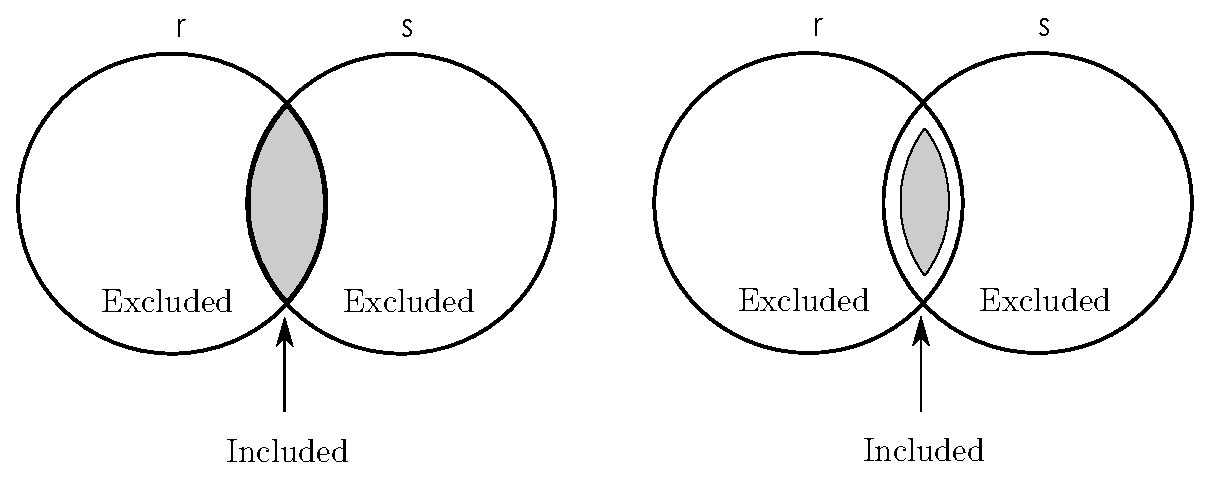
\includegraphics[scale=0.60]{graphs/innerjoin.eps}
\caption{\label{fi:innerjoin} Comparison between the relational (non-temporal) inner join (left graph) and the temporal inner join (right graph).}
\end{figure}



Figure \ref{fi:innerjoin} compares the relational inner join with respect to the temporal inner join. The right graph illustrates the temporal case. It is clear that the temporal inner join is a subset or is equal to the relational inner join.

\subsection{\label{subsec:Equijoin}Equijoin}
The equijoin operator for relational databases enforces equality between specified subsets of the attributes of the relations. Then, the temporal equijoin operator is defined as the temporal join operator.

\begin{definition}
 \label{def:equijoin}
Equijoin. Let $R$ and $S$ be two relations and $r, s$ be the instances of each relation respectively. $A , B$ are the sets of the attributes for the relations $R$ and $D$ respectively. And let $A' \subseteq A$ and $B' \subseteq B$. Then, the temporal equijoin is defined as follows:
\begin{equation}
 \label{eq:equijoin}
R \Join_{r\left[A' \right] = s\left[B' \right]}^{T} S =  \sigma_{r\left[A' \right] = s\left[B' \right]} \left(R \times^T S \right)
\end{equation}
\end{definition}


\subsubsection{\label{subsubsec:temporal-equijoin}Temporal Equijoin}
The temporal equijoin is an equijoin operator in which the subset of attributes in the equijoin condition, are part of the primary key. Hence, the operator is defined as follows:

\begin{definition}
\label{def:temporal-equijoin}
Temporal equijoin ($R$ TE-join $S$). Let $R, S$ be two relations and $r, s$ the instances of each relation respectively. The sets $A, B$ are the attributes of each relation. And $ID \subseteq A; ID \subseteq B$ is the primary key of both relations. The temporal equijoin operator is defined as follows:
\begin{equation}
 \label{eq:temporal-equijoin} 
R \mbox{TE-join} S \equiv R \Join_{r\left[ID\right] = s\left[ID\right]}^{T} S
\end{equation}
\end{definition}

\subsection{\label{subsec:natural-join}Natural Join}
The temporal natural join is a temporal equijoin on identically named attributes.

\begin{definition}
 \label{def:temporal-natural-join}
Temporal natural join. Consider the following relations $R = \left(A_1, \ldots, A_n, C_1, \ldots, C_k, T_s, T_e \right)$ and $S = \left(B_1, \ldots, B_m, C_1, \ldots, C_k, T_s, T_e \right)$. The temporal natural join is defined as follows:
\begin{equation}
 \label{eq:temporal-natural-join}
R \Join^T S = R \Join_{r\left[C_1\right] = s\left[C_1\right] \wedge \ldots \wedge r\left[C_k\right] = s\left[C_k\right]} S
\end{equation}
\end{definition}

\subsection{\label{subsec:outer-joins}Outer Joins}


\begin{figure}
 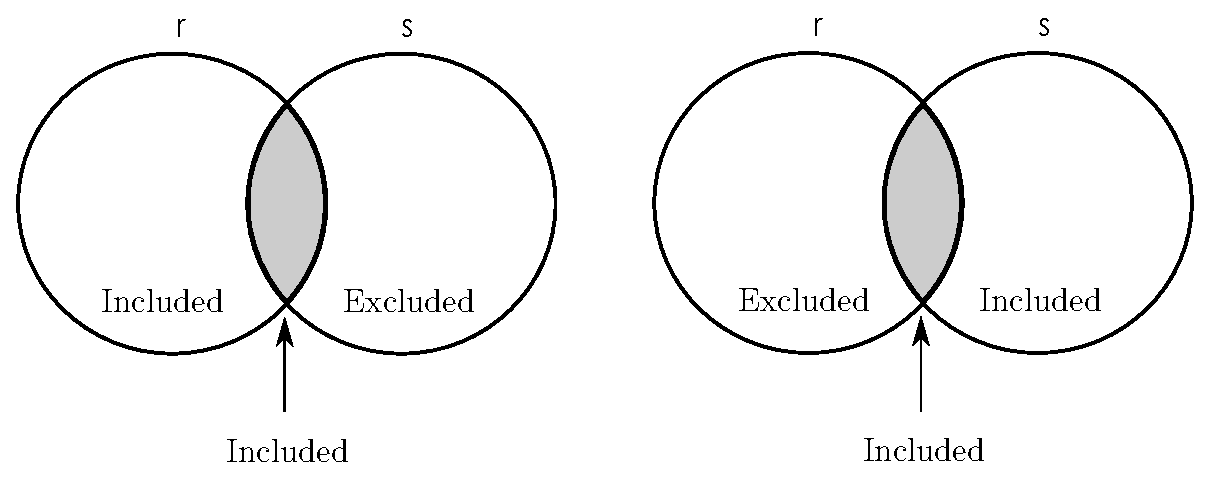
\includegraphics[scale=0.60]{graphs/outerjoin.eps}
\caption{\label{fi:outerjoin} Comparison between a left outer join (left graph) and a right inner join (right graph).}
\end{figure}


%The following example illustrates the behaviour of the join operator in a crisp temporal database.
% \begin{table}
% \centering
% \caption{Join Employees - Address.}
% 
% \begin{tabular}{c c c c c c c c c }
% \hline
% ID & Job & Works for & Start & Finish & Adr. & Start & Finish \\ \hline
% 1 & Prof. & 4 & 5 & 10 & C/ Camino de ronda & - & 12 \\
% \cellcolor[gray]{0.9}
% 1 & \cellcolor[gray]{0.9} Prof. &\cellcolor[gray]{0.9} 4 &\cellcolor[gray]{0.9} 5 &\cellcolor[gray]{0.9} 10 &\cellcolor[gray]{0.9} C/ Manuel de Falla &\cellcolor[gray]{0.9} 12 &\cellcolor[gray]{0.9} - \\ 
% 2 & Tech. & 4 & 3 & 7  & C/ Recogidas & - & - \\ 
% 3 & Account. & 4  & 4 & 10 & C/ Pintor Maldonado & - & - \\
% 4 & Adm. & - & 1 & -& C/ Mesones & - & - \\
% 1 & Prof. & 4 & 11 & - & C/ Manuel de Falla & 12 & - \\
% 1 & Prof. & 4 & 11 & - & C/ Camino de ronda & - & 12 \\
% \hline 
% \end{tabular}
% \label{table:join-employees-address}
% 
% \vspace{10pt}
% 
% 
% \end{table}
% 
% \vspace{-25pt}









\newpage

\section*{Acknowledgements}
%
The researchers are supported by the grant BES-2009-013805 within the research project TIN2008-02066: \emph{Fuzzy Temporal Information treatment in relational DBMS}.

\bibliographystyle{splncs03}
\bibliography{biblio}




\end{document}